\documentclass[10pt]{article}
\usepackage[margin=0.62in]{geometry}
\usepackage{amsmath,amssymb,booktabs,graphicx}
\usepackage[hidelinks]{hyperref}
\setlength{\parindent}{0pt}
\setlength{\parskip}{3pt}
\setlength{\abovedisplayskip}{4pt}
\setlength{\belowdisplayskip}{4pt}
\setlength{\textfloatsep}{7pt}
\setlength{\floatsep}{6pt}
\renewcommand{\arraystretch}{1.08}

\title{\vspace{-1.3cm}\textbf{Controlling $2+2\!\to\!4$ Circuit Formation\\
in a Fully Trainable Two-Block ReLU Network}}
\author{}
\date{\vspace{-1.15cm}}

\begin{document}
\maketitle
\vspace{-0.75cm}

\textbf{Summary.}
We derive a zero-temperature stationary phase diagram for a two-block residual ReLU network
with independent weight decays.  The calculation has two nested levels.  At fixed representation
strengths $(s,q)$, we analytically eliminate the parent readouts, target-producing weights, and
$d4$ readout.  We then minimize the resulting scalar free energy over $(s,q)$ separately for a
direct and a compositional circuit family, and select the family with lower minimum.  The second
block uses a compositional $2+2\to4$ gate when (i) its self-consistent representation satisfies
$Q_2/Q_1^{(1)}>1/\sqrt8$, (ii) the compositional free energy is below the direct one, and
(iii) decay does not suppress the target.  Layerwise decay can control the compositional share,
but it creates a tradeoff: increasing first-block decay suppresses the unwanted first-block
$d4$ shortcut and also suppresses the wanted $d2$ parents.  A compositional phase therefore
exists only inside a finite decay window.

\section*{1. Model and assumptions}
For target parity $\chi_a(x)\in\{-1,+1\}$, let $f_a(x)=w_a^\top h_2(x)$ and define its
target-mode amplitude $\widehat A_a=\mathbb E_x[f_a(x)\chi_a(x)]$.  Under the pure aligned-mode
ansatz $f_a=\widehat A_a\chi_a$, the sample loss reduces as
$\mathbb E_x[(f_a-\chi_a)^2]=(1-\widehat A_a)^2$, since $\chi_a^2=1$.  The network and
reduced weighted objective are therefore
\begin{align}
h_1&=h_0+\sigma(V_1h_0),& h_2&=h_1+\sigma(V_2h_1),\nonumber\\[-2pt]
f_a&=w_a^\top h_2,\nonumber\\[-5pt]
\mathcal J&=\frac{\gamma_2}{2}\!\sum_{a\in\{12,34\}}(1-\widehat A_a)^2
+\frac{\gamma_4}{2}(1-\widehat A_4)^2
+\frac12\!\left(\lambda_E\|E\|^2+\lambda_1\|V_1\|^2+\lambda_2\|V_2\|^2\right.\nonumber\\[-2pt]
&\hspace{4.2cm}\left.+\lambda_p\|W_{d2}\|^2+\lambda_4\|w_4\|^2\right).
\label{eq:objective}
\end{align}
The derivation assumes: (A1) the full four-bit cube and pure ReLU; (A2) four equal-norm,
orthogonal singleton Walsh vectors of norm $s=Q_1^{(0)}$; (A3) two equal-norm, orthogonal
parent vectors $q_{12},q_{34}$ of norm $q=Q_2$; (A4) balanced rank-one gates, sufficient
width, and additive parameter norms for parent and target sectors; (A5) block-1 and block-2
target vectors align with their common readout; (A6) no pre-existing frozen $d4$ feature;
and (A7) the global zero-temperature minimum is reached.  Thus this is an equilibrium
mode theory, not a claim about finite-time SGD or dynamical lock-in.

The symbol $V_1$ in Eq.~\eqref{eq:objective} is the \emph{entire} first-block weight matrix.
Under the additive-sector assumption A4, we decompose it conceptually as
\begin{equation}
V_1=V_{1,\rm parent}+V_{1,d4}+V_{1,\rm other},\qquad
\|V_1\|_F^2=\|V_{1,\rm parent}\|_F^2+
\|V_{1,d4}\|_F^2+\|V_{1,\rm other}\|_F^2.
\label{eq:v1-decomp}
\end{equation}
$V_{1,\rm parent}$ is not a separate network parameter.  It denotes the minimum-norm component
of $V_1$ that implements the two supervised $1+1\to2$ parent gates.  The component
$V_{1,d4}$ implements the direct block-1 target route $D_1$ introduced below.  Their costs can
be minimized separately only because A4 assumes orthogonal sectors and additive squared norms.

The singleton byproduct of an ideal parent gate is not a fitted parameter:
\begin{equation}
\sigma\!\left[a(x_1+x_2)\right]
=\frac a2(1+x_1+x_2+x_1x_2).
\label{eq:relu-decomp}
\end{equation}
It has the same singleton and pair coefficient.  If this generated singleton vector is
orthogonal to the residual singleton vector, then
\begin{equation}
Q_1^{(1)}=\sqrt{s^2+q^2}.
\label{eq:q1out}
\end{equation}
For overlap $\rho$, replace $s^2+q^2$ by $s^2+q^2+2\rho sq$.  All gate-selection statements
below remain exact when expressed using the measured $Q_1^{(1)}$.

\section*{2. Derivation roadmap: what is minimized, and in what order}
The calculation is an algebraic elimination of weights from one simultaneous objective, not a
claim that training executes the following steps in time.  For each candidate target family
$r\in\{H_D,H_C\}$, the minimization is organized as follows.
\begin{enumerate}
\item Choose nonnegative order parameters $(s,q)$, where $s$ fixes the four singleton-feature
norms and $q$ fixes the two $d2$ parent-feature norms.
\item Holding $(s,q)$ fixed, minimize the $d2$ losses and the penalties on $E$,
$V_{1,\rm parent}$, and $W_{d2}$.  This gives the parent-sector free energy $\Phi(s,q)$.
\item Still holding $(s,q)$ fixed, choose either the direct hybrid
$H_D=D_1+D_2$ or the compositional hybrid $H_C=D_1+C$.  Minimize its hidden weights and the
shared $d4$ readout at fixed total target amplitude $A$, then minimize over $A\geq0$.  This
gives the target-sector free energy $G(\zeta_r)$.
\item Finally minimize $\Phi(s,q)+G(\zeta_r)$ over $(s,q)$.  The two families perform this
outer minimization separately, so their optimal representations need not be the same.  The
stationary phase is the family with lower final minimum.
\end{enumerate}
Schematically, the nested calculation is
\begin{equation}
F_r=\min_{s,q\geq0}\left[
\underbrace{\min_{B,\,E,V_{1,\rm parent},W_{d2}}\mathcal J_{d2}}_{\Phi(s,q)}+
\underbrace{\min_{A\geq0,\,\theta_r,w_4}\mathcal J_{d4}}_{G(\zeta_r)}
\right],
\label{eq:roadmap}
\end{equation}
where $B$ is the common fitted amplitude of the two parent targets and $\theta_r$ denotes the
target-producing hidden weights in family $r$.

\section*{3. Eliminating weights: the two stationary free energies}
Equation~\eqref{eq:objective} specifies the penalties but does not by itself imply the norms
below; they are the minimum-norm realizations under A1--A4.  Write $e_i$ for the four
orthogonal singleton vectors.  Then $\|E\|_F^2=\sum_i\|e_i\|^2=4s^2$.  For one balanced
$1+1\to2$ gate of hidden norm $u$, the preactivation amplitude per parent is $us/\sqrt2$;
Eq.~\eqref{eq:relu-decomp} therefore gives $q=us/(2\sqrt2)$, or
$u^2=8q^2/s^2$.  The two disjoint parent gates add in squared norm.  Finally, the
minimum-norm readout satisfying $w_{ij}^{\top}q_{ij}=B$ is
$w_{ij}=Bq_{ij}/q^2$, with $\|w_{ij}\|^2=B^2/q^2$.  Thus the two readout rows also add, giving
\begin{equation}
\|E\|^2=4s^2,\qquad
\|V_{1,\rm parent}\|^2=\frac{16q^2}{s^2},\qquad
\|W_{d2}\|^2=\frac{2B^2}{q^2}.
\end{equation}
At fixed $(s,q)$, the parent-sector objective is therefore
\begin{equation}
\Phi(s,q)\equiv\min_{B\geq0}\left\{
\gamma_2(1-B)^2+2\lambda_Es^2+8\lambda_1\frac{q^2}{s^2}
+\lambda_p\frac{B^2}{q^2}\right\}.
\label{eq:phi-definition}
\end{equation}
This definition includes both $d2$ losses and the regularization needed to create and read out
the singleton and parent representations.  It excludes every $d4$-specific weight and the
$d4$ loss.  Minimizing the displayed expression over the common parent amplitude gives
\begin{align}
B^*(q)&=\frac{\gamma_2q^2}{\gamma_2q^2+\lambda_p},\nonumber\\[-2pt]
\Phi(s,q)&=2\lambda_Es^2+8\lambda_1\frac{q^2}{s^2}
+\frac{\gamma_2\lambda_p}{\gamma_2q^2+\lambda_p}.
\label{eq:parent-free}
\end{align}

There are three target gates: $D_1$ is direct in block 1, $D_2$ is direct in block 2, and
$C$ is compositional in block 2.  Their efficiencies per hidden-weight norm are
\begin{equation}
\eta_{D_1}=\frac{s}{8},\qquad
\eta_{D_2}=\frac{\sqrt{s^2+q^2}}{8},\qquad
\eta_C=\frac{q}{2\sqrt2}.
\label{eq:etas}
\end{equation}
The unrestricted competitors are the aligned hybrids $H_D=D_1+D_2$ and $H_C=D_1+C$.
It is useful to define the inverse hidden-cost factors
\begin{equation}
K_1=\frac{\eta_{D_1}^2}{\lambda_1}=\frac{s^2}{64\lambda_1},\quad
K_{D_2}=\frac{\eta_{D_2}^2}{\lambda_2}=\frac{s^2+q^2}{64\lambda_2},\quad
K_C=\frac{\eta_C^2}{\lambda_2}=\frac{q^2}{8\lambda_2}.
\label{eq:k-factors}
\end{equation}
Larger $K$ means that a route can produce more target amplitude per unit hidden-layer penalty.

Here is the explicit meaning of ``balancing the hidden routes against the readout.''  For
family $r$, let $\mathcal I_D=\{D_1,D_2\}$ or $\mathcal I_C=\{D_1,C\}$.  Let $u_i\geq0$ be
the norm of the target-specific hidden weights assigned to route $i$, and let
$t=\|w_4\|$ be the norm of their shared, aligned readout.  Route $i$ creates hidden target
amplitude $\eta_i u_i$, so the total output amplitude is
$A=t\sum_{i\in\mathcal I_r}\eta_i u_i$.  At fixed $A$, the target-sector regularization is
therefore the constrained minimum
\begin{equation}
\mathcal R_r(A)=
\min_{t,u_i\geq0}\left\{
\frac12\sum_{i\in\mathcal I_r}\lambda_i u_i^2+\frac{\lambda_4}{2}t^2
\;:\; A=t\sum_{i\in\mathcal I_r}\eta_i u_i\right\},
\label{eq:balance-problem}
\end{equation}
where $\lambda_{D_1}=\lambda_1$ and $\lambda_{D_2}=\lambda_C=\lambda_2$.  Define
$K_r=\sum_{i\in\mathcal I_r}\eta_i^2/\lambda_i$.  For fixed $t$, the least-cost allocation is
\begin{equation}
u_i=\frac{A}{tK_r}\frac{\eta_i}{\lambda_i},\qquad
\mathcal R_r(A;t)=\frac{A^2}{2t^2K_r}+\frac{\lambda_4t^2}{2}.
\label{eq:hidden-allocation}
\end{equation}
The first term decreases when the readout is enlarged, while the second increases.  Minimizing
over $t$ makes the two terms equal and gives
\begin{equation}
t^4=\frac{A^2}{\lambda_4K_r},\qquad
\mathcal R_r(A)=A\sqrt{\frac{\lambda_4}{K_r}}=\frac{A}{\zeta_r},qquad
\zeta_r^2\equiv\frac{K_r}{\lambda_4}.
\label{eq:balanced-cost}
\end{equation}
This is the ``balance'': at the optimum, the hidden-route penalty and readout penalty are equal.
It also fixes how the output amplitude is divided among routes:
\begin{equation}
\frac{A_i}{A}=\frac{t\eta_i u_i}{A}
=\frac{\eta_i^2/\lambda_i}{K_r}=\frac{K_i}{K_r}.
\label{eq:route-share}
\end{equation}
For the two candidate families, the effective inverse-cost efficiencies are consequently
\begin{align}
\zeta_D^2&=\frac{K_1+K_{D_2}}{\lambda_4}
=\frac1{\lambda_4}\left[\frac{s^2}{64\lambda_1}
+\frac{s^2+q^2}{64\lambda_2}\right],&
\zeta_C^2&=\frac{K_1+K_C}{\lambda_4}
=\frac1{\lambda_4}\left[\frac{s^2}{64\lambda_1}
+\frac{q^2}{8\lambda_2}\right].
\label{eq:zetas}
\end{align}
After this hidden/readout minimization, only the scalar target-amplitude minimization remains:
\begin{equation}
G(\zeta_r)\equiv\min_{A\geq0}\left\{
\frac{\gamma_4}{2}(1-A)^2+\frac{A}{\zeta_r}\right\}.
\label{eq:g-definition}
\end{equation}
Solving it gives
\begin{align}
A^*(\zeta)&=\left[1-\frac1{\gamma_4\zeta}\right]_+,\nonumber\\[-2pt]
G(\zeta)&=
\begin{cases}
\zeta^{-1}-(2\gamma_4\zeta^2)^{-1},&\gamma_4\zeta>1,\\
\gamma_4/2,&\gamma_4\zeta\leq1.
\end{cases}
\label{eq:target-free}
\end{align}
The closed phase theory is therefore
\begin{equation}
\boxed{F_D=\min_{s,q\geq0}\{\Phi(s,q)+G(\zeta_D)\},\qquad
F_C=\min_{s,q\geq0}\{\Phi(s,q)+G(\zeta_C)\}.}
\label{eq:free-energies}
\end{equation}
Each phase chooses its own representation; the joint-training transition $F_C=F_D$ can
therefore be first order even though the fixed-representation crossover is simple.

\section*{4. Phase diagram and control laws}
At fixed $(s,q)$ the common $D_1$ term cancels, as do $\lambda_2$ and $\lambda_4$:
\begin{equation}
\zeta_C>\zeta_D
\quad\Longleftrightarrow\quad
\frac{q}{\sqrt{s^2+q^2}}=\frac{Q_2}{Q_1^{(1)}}>\frac1{\sqrt8}.
\label{eq:boundary}
\end{equation}
Thus layerwise decay does not directly move the block-2 gate boundary.  It moves the
self-consistent $(s,q)$ and controls how much output goes through block 1.

To define the compositional share, write the fitted target amplitude in the active $H_C$ phase
as $A=A_{D_1}+A_C$, where $A_{D_1}$ is supplied by the direct block-1 route and $A_C$ by the
compositional block-2 route.  We define
\begin{equation}
f_C\equiv\frac{A_C}{A_{D_1}+A_C}.
\label{eq:fc-definition}
\end{equation}
Thus $f_C$ is a share of the signed fitted $d4$ amplitude under the aligned positive-amplitude
ansatz; it is not a fraction of neurons or a probability.  Applying
Eq.~\eqref{eq:route-share} with $K_r=K_1+K_C$ gives
\begin{equation}
\boxed{f_C=\frac{q^2/(8\lambda_2)}{s^2/(64\lambda_1)+q^2/(8\lambda_2)}
=\frac{8\lambda_1q^2}{\lambda_2s^2+8\lambda_1q^2}.}
\label{eq:fraction}
\end{equation}
The number $p\in(0,1)$ is now an externally chosen \emph{purity target}: for example,
$p=1/2$ asks that composition provide a majority of the fitted $d4$ amplitude, whereas
$p=0.9$ asks for a $90\%$ compositional circuit.  It is not another stationarity condition.
Imposing the design requirement $f_C\geq p$ and rearranging Eq.~\eqref{eq:fraction} gives
\begin{align}
f_C\geq p
&\quad\Longleftrightarrow\quad
K_C\geq\frac{p}{1-p}K_1\nonumber\\[-2pt]
&\quad\Longleftrightarrow\quad
\frac{\lambda_1}{\lambda_2}\geq
\frac{p}{1-p}\frac{s^2}{8q^2}.
\label{eq:purity}
\end{align}
But Eq.~\eqref{eq:parent-free} shows that increasing $\lambda_1$ simultaneously makes the
parents more expensive.  The desired circuit therefore requires a window
\begin{equation}
\boxed{\lambda_{1,\rm purity}<\lambda_1<\lambda_{1,\rm parent\ collapse},\quad
F_C<F_D,\quad \gamma_4\zeta_C>1.}
\label{eq:window}
\end{equation}
Here $\lambda_{1,\rm purity}$ is the fixed-$(s,q)$ lower bound from
Eq.~\eqref{eq:purity}, evaluated at the compositional stationary solution, while
$\lambda_{1,\rm parent\ collapse}$ denotes the point at which the outer minimization of
Eq.~\eqref{eq:free-energies} moves to $q=0$, a parents-only solution, or a task-suppressed
solution.  The remaining two conditions say that the compositional family must beat the
direct family globally and that its target amplitude $A^*(\zeta_C)$ must be nonzero.

These are distinct tests: Eq.~\eqref{eq:boundary} chooses the block-2 gate at fixed $(s,q)$;
$F_C<F_D$ chooses the global family after re-optimizing $(s,q)$;
$\gamma_4\zeta_C>1$ makes the $d4$ target active; and $f_C\geq p$ is the analyst's optional
purity threshold.

\begin{figure}[h!]
\centering
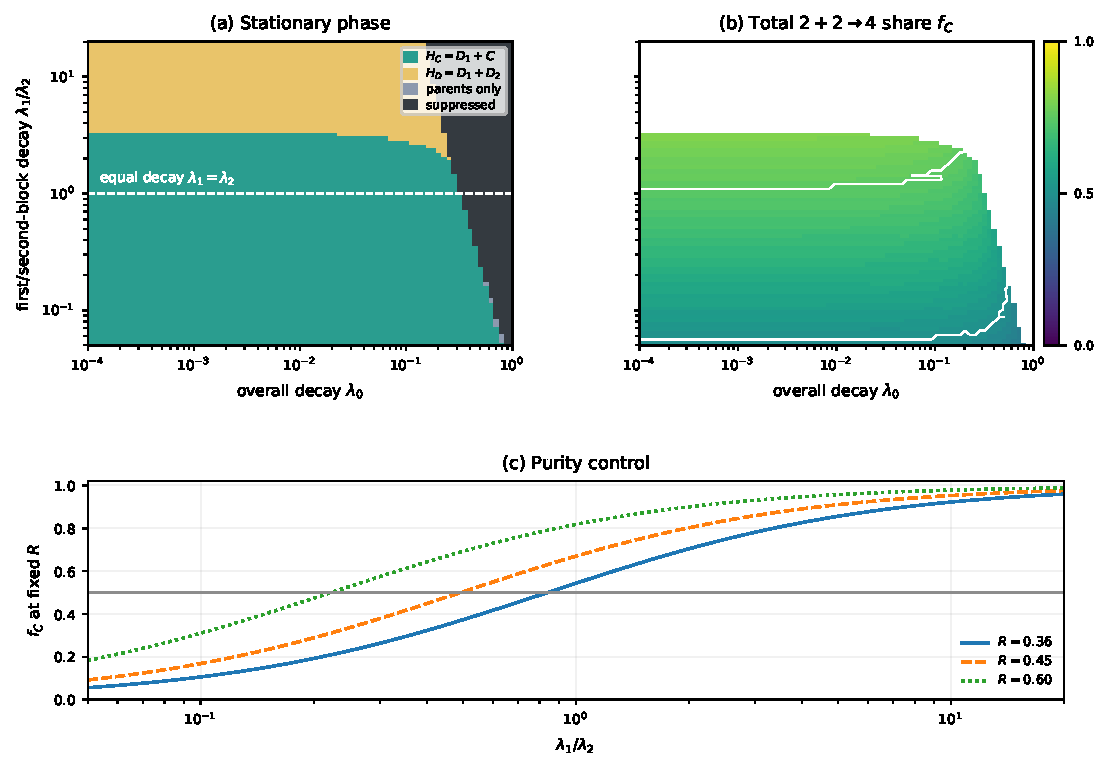
\includegraphics[width=0.99\textwidth]{fig_two_block_layerwise_phase.pdf}
\vspace{-7pt}
\caption{\textbf{Canonical stationary phase diagram.}  We set
$\gamma_2=\gamma_4=2$, $\lambda_E=\lambda_p=\lambda_4=\lambda_2=\lambda_0$,
$\lambda_1/\lambda_2$ as the vertical control, and use assumptions A1--A7.
(a) Global minima of Eq.~\eqref{eq:free-energies}.  Too much first-block decay destroys the
parents and selects $H_D$; sufficiently large overall decay suppresses the tasks.
(b) Composition can be selected yet remain impure when $D_1$ is cheap; white contours mark
the target-amplitude shares $f_C=0.5,0.75,0.9$.  (c) Eq.~\eqref{eq:fraction} at fixed measured accessibility
$R=Q_2/Q_1^{(1)}$: increasing $\lambda_1/\lambda_2$ suppresses the block-1 shortcut, provided
the representation does not fall below Eq.~\eqref{eq:boundary}.}
\label{fig:phase}
\end{figure}

\textbf{How to tune the fully trainable model.}
(1) Decay $w_4$; without it, hidden/readout rescaling invalidates norm comparison.
(2) Preserve the parents with strong $d2$ supervision and modest $\lambda_E,\lambda_1,
\lambda_p$ until the \emph{final} measured $Q_2/Q_1^{(1)}$ exceeds $1/\sqrt8$.
(3) Lower $\lambda_2$ relative to $\lambda_1$ to move target amplitude from $D_1$ into block 2,
then increase $\lambda_1/\lambda_2$ only while the parents remain supercritical.
(4) Measure separately the signed $d4$ readout contributions of $h_1$ and
$\sigma(V_2h_1)$; block-2 neuron classification alone does not measure total circuit share.
(5) If no interval satisfies Eq.~\eqref{eq:window}, whole-layer decay is insufficient:
separate parent-producing and target-specific directions (soft subspace pinning or a decayed
$d4$ adapter).  All weights may remain trainable; freezing is not theoretically required.

\begin{center}
\begin{tabular}{@{}lll@{}}
\toprule
Control & Desired movement & Limiting failure \\
\midrule
$\lambda_1\!\uparrow/\lambda_2$ & $f_C\uparrow$; suppress $D_1$ & parent collapse: $q\downarrow$ \\
$\lambda_2\!\downarrow$ & make block-2 gates cheaper & large block-2 norms \\
$\lambda_p\!\downarrow$ or $\gamma_2\!\uparrow$ & preserve $d2$ parents & weak parent regularization \\
$\lambda_4>0$ & fixes hidden/readout scale & target suppression if too large \\
$\lambda_E\!\downarrow$ & preserve singleton sources & embedding norms grow \\
$\gamma_4\!\uparrow$ & avoids $A^*=0$ & does not by itself select $C$ \\
\bottomrule
\end{tabular}
\end{center}

\textbf{Scope.}
Nonzero singleton overlap $\rho$, unequal parent norms, imperfect target alignment, fixed
block-1 $d4$ leakage, or multifunctional neurons enlarge the order-parameter set but do not
change the measured local boundary in Eq.~\eqref{eq:boundary}.  Finite-temperature Langevin
dynamics replaces $F_C=F_D$ by
$F_C-F_D+\tfrac{T}{2}\log(\det' H_C/\det' H_D)-T\log(g_C/g_D)=0$ and rounds the transition.
Ordinary full-batch SGD is effectively zero-noise but need not reach the global saddle, so
metastability and training history must be checked experimentally.

\end{document}
